% Copyright (c) 2022 by Lars Spreng
% This work is licensed under the Creative Commons Attribution 4.0 International License. 
% To view a copy of this license, visit http://creativecommons.org/licenses/by/4.0/ or send a letter to Creative Commons, PO Box 1866, Mountain View, CA 94042, USA.

%~~~~~~~~~~~~~~~~~~~~~~~~~~~~~~~~~~~~~~~~~~~~~~~~~~~~~~~~~~~~~~~~~~~~~~~~~~~~~~
% You can add your packages and commands to the loadslides.tex file. 
% The files in the folder "styles" can be modified to change the layout and design of your slides.
% I have included examples on how to use the template below. 
% Some of it these examples are taken from the Metropolis template.
%~~~~~~~~~~~~~~~~~~~~~~~~~~~~~~~~~~~~~~~~~~~~~~~~~~~~~~~~~~~~~~~~~~~~~~~~~~~~~~


\documentclass[12pt,notheorems,hyperref={pdfauthor=whatever}]{beamer}


% Copyright (c) 2022 by Lars Spreng
% This work is licensed under the Creative Commons Attribution 4.0 International License. 
% To view a copy of this license, visit http://creativecommons.org/licenses/by/4.0/ or send a letter to Creative Commons, PO Box 1866, Mountain View, CA 94042, USA.

%~~~~~~~~~~~~~~~~~~~~~~~~~~~~~~~~~~~~~~~~~~~~~~~~~~~~~~~~~~~~~~~~~~~~~~~~~~~~~~
% Add your packages and commands to this file
%~~~~~~~~~~~~~~~~~~~~~~~~~~~~~~~~~~~~~~~~~~~~~~~~~~~~~~~~~~~~~~~~~~~~~~~~~~~~~~

%~~~~~~~~~~~~~~~~~~~~~~~~~~~~~~~~~~~~~~~~~~~~~~~~~~~~~~~~~~~~~~~~~~~~~~~~~~~~~~
\RequirePackage{palatino}
\RequirePackage[utf8]{inputenc}
\RequirePackage[T1]{fontenc}
\usepackage{hyperref}
\usepackage{fontawesome}

\usefonttheme{serif}

\usepackage{styles/elegantmacros}
\usefolder{styles}
\usetheme[style=blue]{elegant}

\newcommand{\makepart}[1]{ % For convenience
\part{#1} \frame{\partpage}
}

%~~~~~~~~~~~~~~~~~~~~~~~~~~~~~~~~~~~~~~~~~~~~~~~~~~~~~~~~~~~~~~~~~~~~~~~~~~~~~~

%~~~~~~~~~~~~~~~~~~~~~~~~~~~~~~~~~~~~~~~~~~~~~~~~~~~~~~~~~~~~~~~~~~~~~~~~~~~~~~
% Figures
\RequirePackage{booktabs}
\RequirePackage{colortbl}
\RequirePackage{ragged2e}
\RequirePackage{schemabloc}
%\RequirePackage{natbib}
\RequirePackage{caption}
\RequirePackage{subcaption}
\RequirePackage{tabularx}
\RequirePackage{array}
\RequirePackage{multirow}
\usepackage[alf, bibjustif]{abntex2cite}
\newcolumntype{Y}{>{\centering\arraybackslash}X}

%~~~~~~~~~~~~~~~~~~~~~~~~~~~~~~~~~~~~~~~~~~~~~~~~~~~~~~~~~~~~~~~~~~~~~~~~~~~~~~

%~~~~~~~~~~~~~~~~~~~~~~~~~~~~~~~~~~~~~~~~~~~~~~~~~~~~~~~~~~~~~~~~~~~~~~~~~~~~~~
% Figures
\RequirePackage{wrapfig}
\RequirePackage{pgfplots}
\RequirePackage{graphicx}
\RequirePackage{adjustbox}
\RequirePackage{environ}
\pgfplotsset{compat=1.18}

\makeatletter
\newsavebox{\measure@tikzpicture}
\NewEnviron{scaletikzpicturetowidth}[1]{%
  \def\tikz@width{#1}%
  \def\tikzscale{1}\begin{lrbox}{\measure@tikzpicture}%
  \BODY
  \end{lrbox}%
  \pgfmathparse{#1/\wd\measure@tikzpicture}%
  \edef\tikzscale{\pgfmathresult}%
  \BODY
}
\makeatother
%~~~~~~~~~~~~~~~~~~~~~~~~~~~~~~~~~~~~~~~~~~~~~~~~~~~~~~~~~~~~~~~~~~~~~~~~~~~~~~

%~~~~~~~~~~~~~~~~~~~~~~~~~~~~~~~~~~~~~~~~~~~~~~~~~~~~~~~~~~~~~~~~~~~~~~~~~~~~~~
% Maths 
\RequirePackage{textcomp}
\RequirePackage{amsmath} 
\RequirePackage{amsthm}
\RequirePackage{mathtools}
%\RequirePackage{bbm}
%\RequirePackage{algorithm}
%\RequirePackage[osf,sc]{mathpazo}
%\RequirePackage{pifont}
%\newcommand{\xmark}{\ding{55}}%
%\numberwithin{equation}{section}
\DeclareMathOperator*{\argmax}{arg\,max}
\DeclareMathOperator*{\argmin}{arg\,min}

\setbeamertemplate{theorems}[numbered] % to number

\theoremstyle{definition}
\newtheorem{fact}{Fact}[section]
\newtheorem{examp}{Example}[section]

\theoremstyle{plain}
\newtheorem{definition}{Definition}[section]
\newtheorem{proposition}{Proposition}
\newtheorem{theorem}{Theorem}
\newtheorem{assumption}{Assumption}

\providecommand{\H}{\mathscr{H}}      
\providecommand{\E}{\mathbb{E}}
\makeatletter
\def\munderbar#1{\underline{\sbox\tw@{$#1$}\dp\tw@\z@\box\tw@}}
\makeatother

%~~~~~~~~~~~~~~~~~~~~~~~~~~~~~~~~~~~~~~~~~~~~~~~~~~~~~~~~~~~~~~~~~~~~~~~~~~~~~~
 % Loads packages and some defined commands


\usepackage{amsmath,scalerel}

\DeclareMathOperator*{\concat}{\scalerel*{\Vert}{\sum}}

\title[
% Text entered here will appear in the bottom middle
]{\textit{Graph Transformer Networks}}

\subtitle{\cite{DBLP:journals/corr/abs-1911-06455}}

\author[
% Text entered here will appear in the bottom left corner
]{
    Ana Carolina Erthal e Felipe Lamarca
}


\institute{
    Escola de Matemática Aplicada \\
    Fundação Getulio Vargas}
\date{}

\begin{document}

% Generate title page
{
\setbeamertemplate{footline}{} 
\begin{frame}
  \titlepage
\end{frame}
}
\addtocounter{framenumber}{-1}

% You can declare different parts as a parentof sections
\begin{frame}{Estrutura da apresentação}
    \tableofcontents
\end{frame}

%%%%%%%%%%%%%%%%%%%%%%%%%%%%%%%%%%%%%%%%%%
%%%%%%%%%%%%%%%%%%%%%%%%%%%%%%%%%%%%%%%%%%
%%%%%%%%%%%%%%%%%%%%%%%%%%%%%%%%%%%%%%%%%%
%%%%%%%%%%%%%%%%%%%%%%%%%%%%%%%%%%%%%%%%%%

\section{Introdução}

%%%%%%%%%%%%%%%%%%%%%%%%%%%%%%%%%%%%%%%%%%

\subsection{Estado da arte}
\begin{frame}

    Para prever arestas e classificar nós e grafos, normalmente usa-se \underline{Graph Neural Networks} (GNNs).
    
    \vspace{10pt}

    Esse modelo, no entanto, assume que os \textbf{grafos são homogêneos}, o que não é verdade em muitos casos.

    \vspace{10pt}


    \begin{description}
        \item[\textbf{Grafos de citações são heterogêneos}]
    \end{description}
    \begin{itemize}
        \item Nós representam Autores, Papers, Conferências
        \item Arestas representam relações do tipo Autor-Paper, Paper-Conferência
    \end{itemize}

    \vspace{10pt}


    Uma abordagem naive é ignorar esses tipos e tratar todos os grafos como homogêneos, o que é uma abordagem sub-ótima na medida em que implica perda de informação.

    
    % \href{https://github.com/anacarolerthal/conformal-prediction-evaluation}{\faicon{github}  Repositório do \textit{paper}}
\end{frame}

%%%%%%%%%%%%%%%%%%%%%%%%%%%%%%%%%%%%%%%%%%

\subsection{Soluções anteriores}
\begin{frame}

Para contornar  problema, é comum...

\begin{enumerate}
    \item Pré-processar o grafo para transformá-lo em homogêneo
    \item Aplicar uma GNN em seguida
\end{enumerate}

    \vspace{10pt}

    \begin{description}
        \item[\textbf{Pré-processamento através de meta-paths}]
    \end{description}
    \begin{itemize}
        \item Relações compostas entre diferentes tipos de nó
        \item Selecionados manualmente caso a caso
        \item Escolhas ruins de meta-paths podem levar a resultados ruins
    \end{itemize}

    \vspace{10pt}
    
    
    
\end{frame}
%%%%%%%%%%%%%%%%%%%%%%%%%%%%%%%%%%%%%%%%%%%
\begin{frame}
    
\begin{figure}
    \centering
    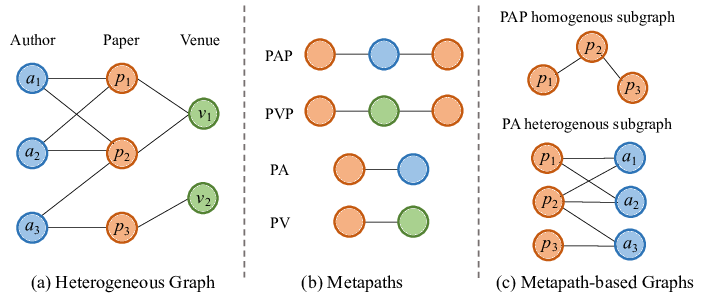
\includegraphics[width=480pt]{img/image_metapath.png}
    \caption{\cite{cai_2021}}
    \label{fig:metapath}
\end{figure}

    
\end{frame}

%%%%%%%%%%%%%%%%%%%%%%%%%%%%%%%%%%%%%%%%%%

\subsection{Graph Transformer Networks}
\begin{frame}
    A solução trazida pela \textbf{GTN} é um framework end-to-end que:
    \begin{enumerate}
        \item Aprende a transformar grafos heterogêneos em homogêneos, identificando meta-paths úteis de acordo com a tarefa em questão
        \item Aprende \textit{node representations} no grafo transformado através de uma GNN para poder realizar a tarefa.        
    \end{enumerate}
\end{frame}

%%%%%%%%%%%%%%%%%%%%%%%%%%%%%%%%%%%%%%%%%%
%%%%%%%%%%%%%%%%%%%%%%%%%%%%%%%%%%%%%%%%%%
%%%%%%%%%%%%%%%%%%%%%%%%%%%%%%%%%%%%%%%%%%
%%%%%%%%%%%%%%%%%%%%%%%%%%%%%%%%%%%%%%%%%%

\section{Metodologia}
% \subsection{Ideia geral}
% \begin{frame}

%     \textbf{IDEIA}: gerar novas estruturas de grafo e, ao mesmo tempo, aprender as representações de nós dessas estruturas.

%     \vspace{10pt}

%     \textbf{COMO:} 

%     \vspace{10pt}
    
%     (no lugar das abordagens anteriores, que assumem que o grafo é dado...)

%     \vspace{10pt}
    
%     Usa GTN para obter novos grafos a partir de \underline{múltiplos candidatos a matriz de adjacência} para realizar convoluções e aprender node representations mais poderosas.

% \end{frame}

\subsection{Definições}
\begin{frame}

    \begin{definition}[Grafo heterogêneo]
        $\mathcal{G} = (\mathcal{V}, \mathcal{E}, \mathcal{T}^{v}, \mathcal{T}^{e})$ é um grafo direcionado onde cada nó $v \in \mathcal{V}$ e cada aresta $e \in \mathcal{E}$ estão associadas às suas respectivas funções de mapeamento de tipo $f_v: V \rightarrow \mathcal{T}^v$ e $f_e: \mathcal{E} \rightarrow \mathcal{T}^e$. \\
        
        Quando $|\mathcal{T}^e| = 1$ e $|\mathcal{T}^v| = 1$, trata-se de um grafo homogêneo. Trataremos do caso $|\mathcal{T}^e| > 1$. 

        \vspace{10pt}
        
        Seja $N$ o número de nós do grafo. O grafo heterogêneo pode ser representado por um conjunto de matrizes de adjacência $\{A_k\}^K_{k=1}$, onde $K = |\mathcal{T}^e|$, e $A_k \in \mathbf{R}^{N \times N}$ é a matriz de adjacência onde $A_k[i, j]$ é não-nulo quando há uma aresta do tipo $k$ entre $j$ e $i$. De maneira mais concisa, o grafo heterogêneo pode ser escrito como o tensor $\mathbb{A} \in \mathbf{R}^{N \times N \times K}$.
    \end{definition}

\end{frame}
%%%%%%%%%%%%%%%%%%%%%%%%%%%%%%%%%%%%%%%%%

\begin{frame}

    \begin{definition}[Meta-path]
        Meta-path ($p$): caminho em um grafo heterogêneo, dado por 
        $v_1 \xrightarrow{t_1} v_2 \xrightarrow{t_2} ... \xrightarrow{t_l} v_{l+1}$, $t_l \in \mathcal{T}^{e}$. \\
        \vspace{5pt}
        Para uma sequência de tipos de aresta $(t_1, t_2, ..., t_l)$, a matriz de adjacência do meta-path definido por essa sequência é dada por $$A_p= A_{t_l} ... A_{t_2}A_{t_1}$$
    \end{definition}

    \begin{itemize}
        \item     Por exemplo, o meta-path APC (Autor-Paper-Conferência) é do tipo $\text{A}\xrightarrow{AP}\text{P}\xrightarrow{PC}\text{C}$, e a matriz de adjacência do meta-path $A_{APC}=A_{PC}A_{AP}$
    \end{itemize}
\end{frame}

%%%%%%%%%%%%%%%%%%%%%%%%%%%%%%%%%%%%%%
\subsection{Graph Convolutional Network}

\begin{frame}
    Uma \textbf{GCN} é utilizada para aprender $\textit{node representations}$ após já termos as matrizes de adjacência dos meta-paths aprendidos para o grafo $\mathcal{G}$. O \textit{forward propagation} da nossa GCN será:

    $$H^{(l+1)} = \sigma(\Tilde{D}^{\frac{1}{2}} \Tilde{A}\Tilde{D}^{\frac{1}{2}}H^{(l)}W^{(l)}),$$

    onde $\Tilde{A}=A+I$, adicionando \textit{self-connections}, $\Tilde{D}= \sum_i \Tilde{A}_{ij}$ e $W$ é uma matriz de pesos treinável.

    \vspace{15pt}

    \begin{itemize}
        \item Na prática, a camada de convolução é dada pela composição de uma parte fixa e uma transformação linear dos nós.
        \item Além disso, como veremos a seguir, $A$ representa múltiplos meta-paths, então nos beneficiamos de várias estruturas de grafo.
        \item Usamos grafos direcionados, então adaptamos para $H^{(l+1)} = \sigma(\Tilde{D}^{-1} \Tilde{A}H^{(l)}W^{(l)})$
    \end{itemize}
\end{frame}



%%%%%%%%%%%%%%%%%%%%%%%%%%%%%%%%%%%%%%
\subsection{Geração de Meta-Paths}
\begin{frame}
    \begin{columns}
    \column{0.35\textwidth}
    \begin{itemize}
        \scriptsize
        \item A Graph Transformer Layer escolhe duas estruturas de grafo a partir de $\mathbb{A}$ aplicando a \textit{softmax} nos pesos iniciais.

        \vspace{5pt}
        
        Cada layer da GTN aprende a escolher matrizes de adjacência (tipos de arestas) através de uma convolução $1 \times 1$ com os pesos da softmax:
        
        $$
        \begin{align*}
            Q &= F(\mathbb{A}; \phi^{(k)}) \\
              &= \text{conv}_{1 \times 1}(\mathbb{A}; \text{softmax}(\phi^{(k)})) \\
              &= \sum^{|\mathcal{T}_e|}_{t=1} \alpha_t^{(k)} A_t,
        \end{align*} 
        $$

        onde $\phi^{(k)} \in \mathbf{R}^{1\times1\times |\mathcal{T}^e|}$ é o parâmetro da convolução e $\alpha^{(k)} = \text{softmax}(\phi^{(k)})$. Na prática, uma combinação linear das matrizes de adjacência. 

        \vspace{5pt}
        
        \item Multiplica as duas matrizes para obter uma nova estrutura de grafo.
        
    \end{itemize}
    
    \column{0.65\textwidth}
    \begin{figure}
        \centering
        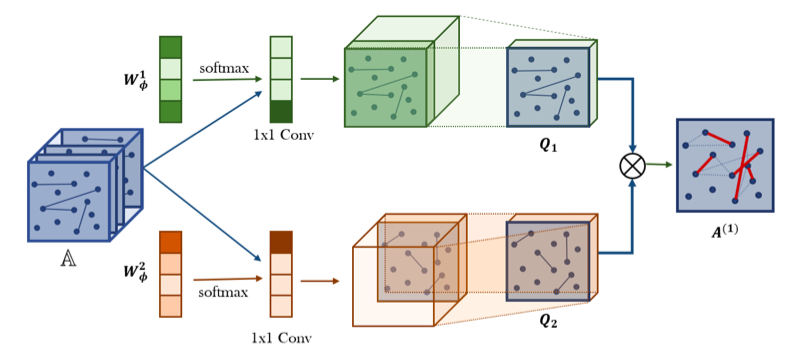
\includegraphics[width=10cm]{img/gt-layer.png}
        \caption{Graph Transformer Layer, \cite{DBLP:journals/corr/abs-1911-06455}}
        \label{fig:gt-layer}
    \end{figure}
    \end{columns}

\end{frame}

\begin{frame}
    A matriz de adjacência de meta-paths de tamanho $l$ é dada por:

    $$A_p = \left( \sum_{t_1 \in \mathcal{T}^e} \alpha_{t_1}^{(1)}A_{t_1}\right)\left( \sum_{t_2 \in \mathcal{T}^e} \alpha_{t_2}^{(2)}A_{t_2}\right)...\left( \sum_{t_l \in \mathcal{T}^e} \alpha_{t_l}^{(l)}A_{t_l}\right)$$

    Assim, com $l$ layers conseguimos aprender meta-paths de tamanho $l$.

\vspace{15pt}

    \begin{itemize}
        \item Uma questão é que adicionando uma layer, aumentamos o tamanho do meta-path, e às vezes é bom ter meta-paths curtos. Por isso, incluímos $A_0 = I$ em $\mathbb{A}$.
    \end{itemize}
\end{frame}

%%%%%%%%%%%%%%%%%%%%%%%%%%%%%%%%%%%%%%%%%%

\section{Graph Transformer Network}
\begin{frame}

\begin{figure}
    \centering
    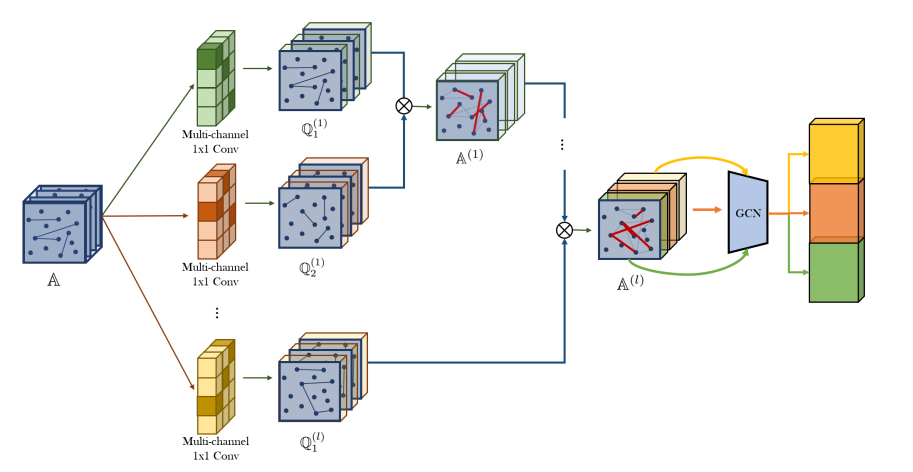
\includegraphics[width=460pt]{img/gt-complete.png}
    \caption{Graph Transformer Network, \cite{DBLP:journals/corr/abs-1911-06455}}
    \label{fig:gtn}
\end{figure}

\end{frame}



\begin{frame}
Para considerarmos vários meta-paths simultaneamente, utilizamos convoluções 1 $\times$ 1 com output de tamanho $C$, sendo $C$ o número desejado de meta-paths.

\begin{itemize}
    \item Isso é útil porque queremos aprender \textit{node representations} a partir de várias estruturas de grafos, para que haja mais "tentativas" de adequação à tarefa. 
\end{itemize}


\vspace{10pt}

Sendo assim, após $l$ GT layers, aplicamos uma GCN a cada canal  matriz $\mathbb{A}$ de meta-paths, e concatenamos os \textit{node representations} obtidos:
$$Z =\concat_{i=1}^C\sigma(\Tilde{D}_i^{-1} \Tilde{A}_i^{(l)}XW),$$

onde $W$ é uma matriz de pesos compartilhada entre os canais e $X$ é a matriz de features para cada nó.

\vspace{10pt}

Tendo \textit{node representations}, podemos incluir camadas densas para realizar classificações.
\end{frame}

%%%%%%%%%%%%%%%%%%%%%%%%%%%%%%%%%%%%%%%%%%

\section{Experimentos}

\begin{frame}
    \begin{figure}
        \centering
        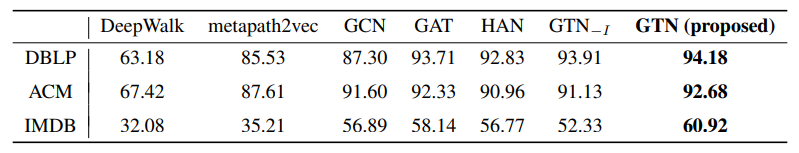
\includegraphics[width=15cm]{img/experiments.png}
        \caption{Resultados na tarefa de classificação de nós (F1-score), \cite{DBLP:journals/corr/abs-1911-06455}}
        \label{fig:enter-label}
    \end{figure}
    
\end{frame}


\begin{frame}
    \begin{figure}
        \centering
        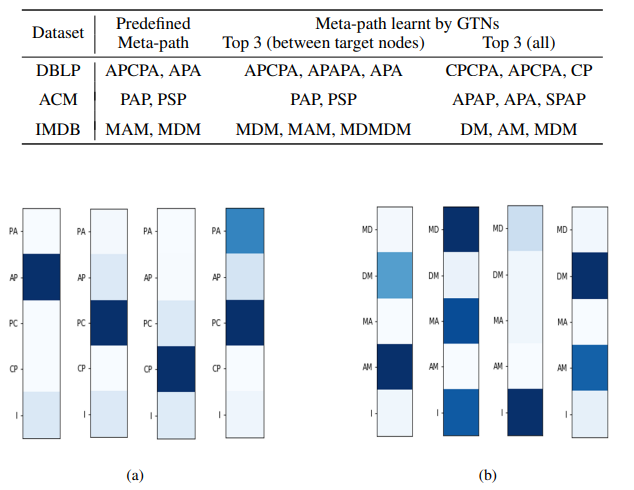
\includegraphics[width=10cm]{img/attention.png}
        \caption{Meta-paths e atenção obtidos pelo GTN em comparação a meta-paths pré-definidos
        \cite{DBLP:journals/corr/abs-1911-06455}}
        \label{fig:attention}
    \end{figure}
    
\end{frame}

%%%%%%%%%%%%%%%%%%%%%%%%%%%%%%%%%%%%%%%%%%
%%%%%%%%%%%%%%%%%%%%%%%%%%%%%%%%%%%%%%%%%%


\section{Referências bibliográficas}
\begin{frame}
    \nocite{DBLP:journals/corr/abs-1911-06455}
    \nocite{YUN2022104}
    \nocite{cai_2021}
    \bibliography{references}
\end{frame}
\end{document}

%%%%%%%%%%%%%%%%%%%%%%%%%%%%%%%%%%%%%%%%%%
%%%%%%%%%%%%%%%%%%%%%%%%%%%%%%%%%%%%%%%%%%
%%%%%%%%%%%%%%%%%%%%%%%%%%%%%%%%%%%%%%%%%%
%%%%%%%%%%%%%%%%%%%%%%%%%%%%%%%%%%%%%%%%%%